\documentclass{beamer} 
\usepackage{amsmath,amsthm}
\usepackage{graphicx,microtype,parskip}
\usepackage{caption,subcaption,multirow}
\usepackage{attrib}

\frenchspacing

\usetheme{default}
\usecolortheme{whale}

\setbeamertemplate{navigation symbols}{}

\setbeamercolor{title}{fg=blue,bg=white}

\setbeamercolor{block title}{fg=white,bg=gray}
\setbeamercolor{block body}{fg=black,bg=lightgray}

\setbeamercolor{block title alerted}{fg=white,bg=darkgray}
\setbeamercolor{block body alerted}{fg=black,bg=lightgray}

%\AtBeginSection[]
%{
%  \begin{frame}
%    \tableofcontents[currentsection]
%  \end{frame}
%}

\title{Death and Taxa}
\subtitle{time-invariant differences in mammal species durations}
\author{Peter D Smits}
\institute{Committee on Evolutionary Biology, University of Chicago}
\titlegraphic{
  \includegraphics[width=2.75cm,height=2.75cm,keepaspectratio=true]{figure/paleodb}
  \hspace*{0.35\paperwidth}
  \includegraphics[width=2cm,height=2cm,keepaspectratio=true]{figure/chicago}
}
\date{}

\begin{document}

\begin{frame}
  \maketitle
\end{frame}

\begin{frame}
  \begin{alertblock}{Question}
    Why do taxa go extinct at different rates?
  \end{alertblock}
\end{frame}

\begin{frame}
  \begin{block}{Motivating questions}
    \begin{itemize}
      \item How do mammal species traits affect extinction risk?
        \begin{itemize}
          \item How do shared time of origination or evolutionary history relate to extinction risk?
        \end{itemize}
      \item How do my findings compare to current risk factors?
      \item Is species extinction risk age-independent?
    \end{itemize}
  \end{block}
\end{frame}

\begin{frame}
  \begin{block}{Motivating questions}
    \begin{itemize}
      \item \alert{How do mammal species traits affect extinction risk?}
        \begin{itemize}
          \item \alert{How do shared time of origination or evolutionary history relate to extinction risk?}
        \end{itemize}
      \item How do my findings compare to current risk factors?
      \item Is species extinction risk age-independent?
    \end{itemize}
  \end{block}
\end{frame}

\begin{frame}
  \frametitle{Relationship between range size and extinction risk}
  \begin{center}
    \includegraphics[width = \textwidth,height = 0.8\textheight,keepaspectratio = true]{figure/harnik_rarity}
  \end{center}
  
  \tiny{\attrib{Harnik and Simpson 2013 \textit{Proc B}}}
\end{frame}

\begin{frame}
  \frametitle{Survival of the unspecialized}
  \begin{quote}
    When related phyla die out \dots more specialized phyla tend to become extinct before less specialized. This phenomenon is also far from universal, but it is so common that it does deserve recognition as a rule or principle in evolutionary studies: \textbf{the rule of the survival of the relatively unspecialized.}

    \small{\attrib{Simpson, 1944, \em{Tempo and Mode of Evolution}, p. 143}}
  \end{quote}
\end{frame}

\begin{frame}
  \frametitle{Hypotheses of effects of dietary category}
  \begin{center}
    \includegraphics[width = \textwidth,height = 0.8\textheight,keepaspectratio = true]{figure/diet_survival}
  \end{center}
\end{frame}

\begin{frame}
  \frametitle{Hypotheses of effects of locomotor category}
  \begin{center}
    \includegraphics[width = \textwidth,height = 0.8\textheight,keepaspectratio = true]{figure/loco_initial}
  \end{center}
\end{frame}

\begin{frame}
  \frametitle{Hypotheses of effects of locomotor category}
  \begin{center}
    \includegraphics[width = \textwidth,height = 0.8\textheight,keepaspectratio = true]{figure/loco_later}
  \end{center}
\end{frame}

\begin{frame}
  \frametitle{Hierarchical Bayesian modeling approach}

  \includegraphics[width = \textwidth,height = 0.8\textheight,keepaspectratio = true]{figure/han_bayes}

  \tiny{\attrib{www.countbayesie.com}}
\end{frame}

\begin{frame}
  \frametitle{Survival model diagram}
  \begin{center}
    \includegraphics[height=0.8\textheight,keepaspectratio=true]{figure/mammal_model}
  \end{center}
\end{frame}

\begin{frame}
  \frametitle{Pattern of species survival under two models}
  
  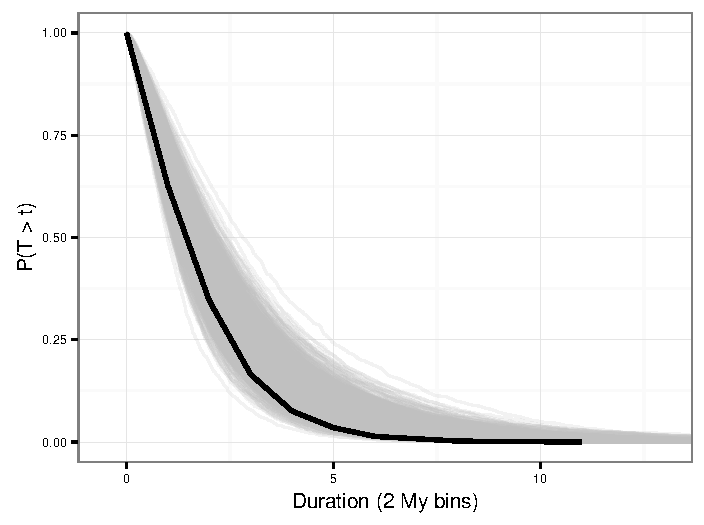
\includegraphics[height=0.8\textheight,keepaspectratio=true]{figure/survival_function_pres}
\end{frame}

\begin{frame}
  \frametitle{Effect of dietary category on extinction risk}
  
  \includegraphics[height=0.8\textheight,keepaspectratio=true]{figure/diet_diff_est_pres}
\end{frame}

\begin{frame}
  \frametitle{Effect of locomotor category on extinction risk}
  
  \includegraphics[height=0.8\textheight,keepaspectratio=true]{figure/loco_diff_est_pres}
\end{frame}

\begin{frame}
  \frametitle{Difference in risk between origination cohorts}
  
  \includegraphics[height=0.8\textheight,keepaspectratio=true]{figure/cohort_est_pres}
\end{frame}

\begin{frame}
  \frametitle{Three sources of variance}
  
  \includegraphics[height=0.8\textheight,keepaspectratio=true]{figure/variance_est_pres}
\end{frame}

\begin{frame}
  \begin{block}{Conclusions}
    \begin{itemize}
      \item Survival of the unspecialized as time-invariant generalization.
      \item Decrease in extinction risk with time.
        \begin{itemize}
          \item Both cohort/temporal and phylogenetic effect.
        \end{itemize}
      \item Some incongruence with risk factors in the Recent.
        \begin{itemize}
          \item e.g. effect of body size, trophic category, phylogenetic clustering.
        \end{itemize}
    \end{itemize}
  \end{block}
\end{frame}

\begin{frame}
  \frametitle{Acknowledgements}
  \begin{columns}
    \begin{column}{0.5\textwidth}
      \begin{itemize}
        \item Advising
          \begin{itemize}
            \item Kenneth D. Angielczyk, Michael J. Foote, \\P. David Polly, \\Richard H. Ree
          \end{itemize}
        \item Angielczyk Lab
          \begin{itemize}
            \item {\small{David Grossnickle, \\Dallas Krentzel}}
          \end{itemize}
        \item Foote lab
          \begin{itemize}
            \item {\small{Marites Villarosa Garcia, \\Nadia Pierrehumbert, \\Kathleen Ritterbush}}
          \end{itemize}
      \end{itemize}
    \end{column}
    \begin{column}{0.5\textwidth}
      \begin{itemize}
        \item {\footnotesize{Stewart Edie, \\Colin Kyle, \\Darcy Ross, \\Elizabeth Sander, \\Laura Southcott, \\Courtney Stepien}}
        \item {\footnotesize{John Alroy, \\David Bapst, \\Ben Frable, \\Graeme Lloyd, \\Carl Simpson, \\Graham Slater, \\Peter Wagner}}
      \end{itemize}
    \end{column}
  \end{columns}
\end{frame}

\appendix

\begin{frame}
  \frametitle{Further posterior predictive checks}
  
  \includegraphics[height=0.8\textheight,keepaspectratio=true]{figure/quant_ppc_pres}
\end{frame}

%\begin{frame}
%  \frametitle{Model specifications}
%
  % ~ 2000 species
  % phylogeny is mostly based on taxonomy
  %   mbl time scaling w/ 0.1 My added to zlb-s
  %
  % inference in STAN, 30000 steps, evaluate chain mixing via Rhat
%\end{frame}

\begin{frame}
  \frametitle{Concerns regarding estimation of \(\alpha\)}
  
  \includegraphics[height=0.8\textheight,keepaspectratio=true]{figure/alpha_simulation}
\end{frame}

\end{document}
